\section{Introduction}
\label{sec:Introduction}

\subsection{Background}
Generating content for large computer games or CGI effects in feature films is a significant bottleneck in terms of effort and resources. A typical game contains many thousands of audio files, images, textures and 3D models. Procedurally generated content provides a cost-effective alternative to the manual creation of models, textures, images and sound assets and can expand playability beyond what is otherwise possible. The video game "No Man's Sky", for example, was released in 2016 and relies on procedural asset generation to create over 18 quintillion planets each of which has a unique ecosystem composed of flora and fauna. Figure \ref{Screenshot NoManSky} is a screenshot of "No Man's Sky". Such a scale is, of course, beyond the reach of any manually created system.

\begin{figure}[htb]
\centering
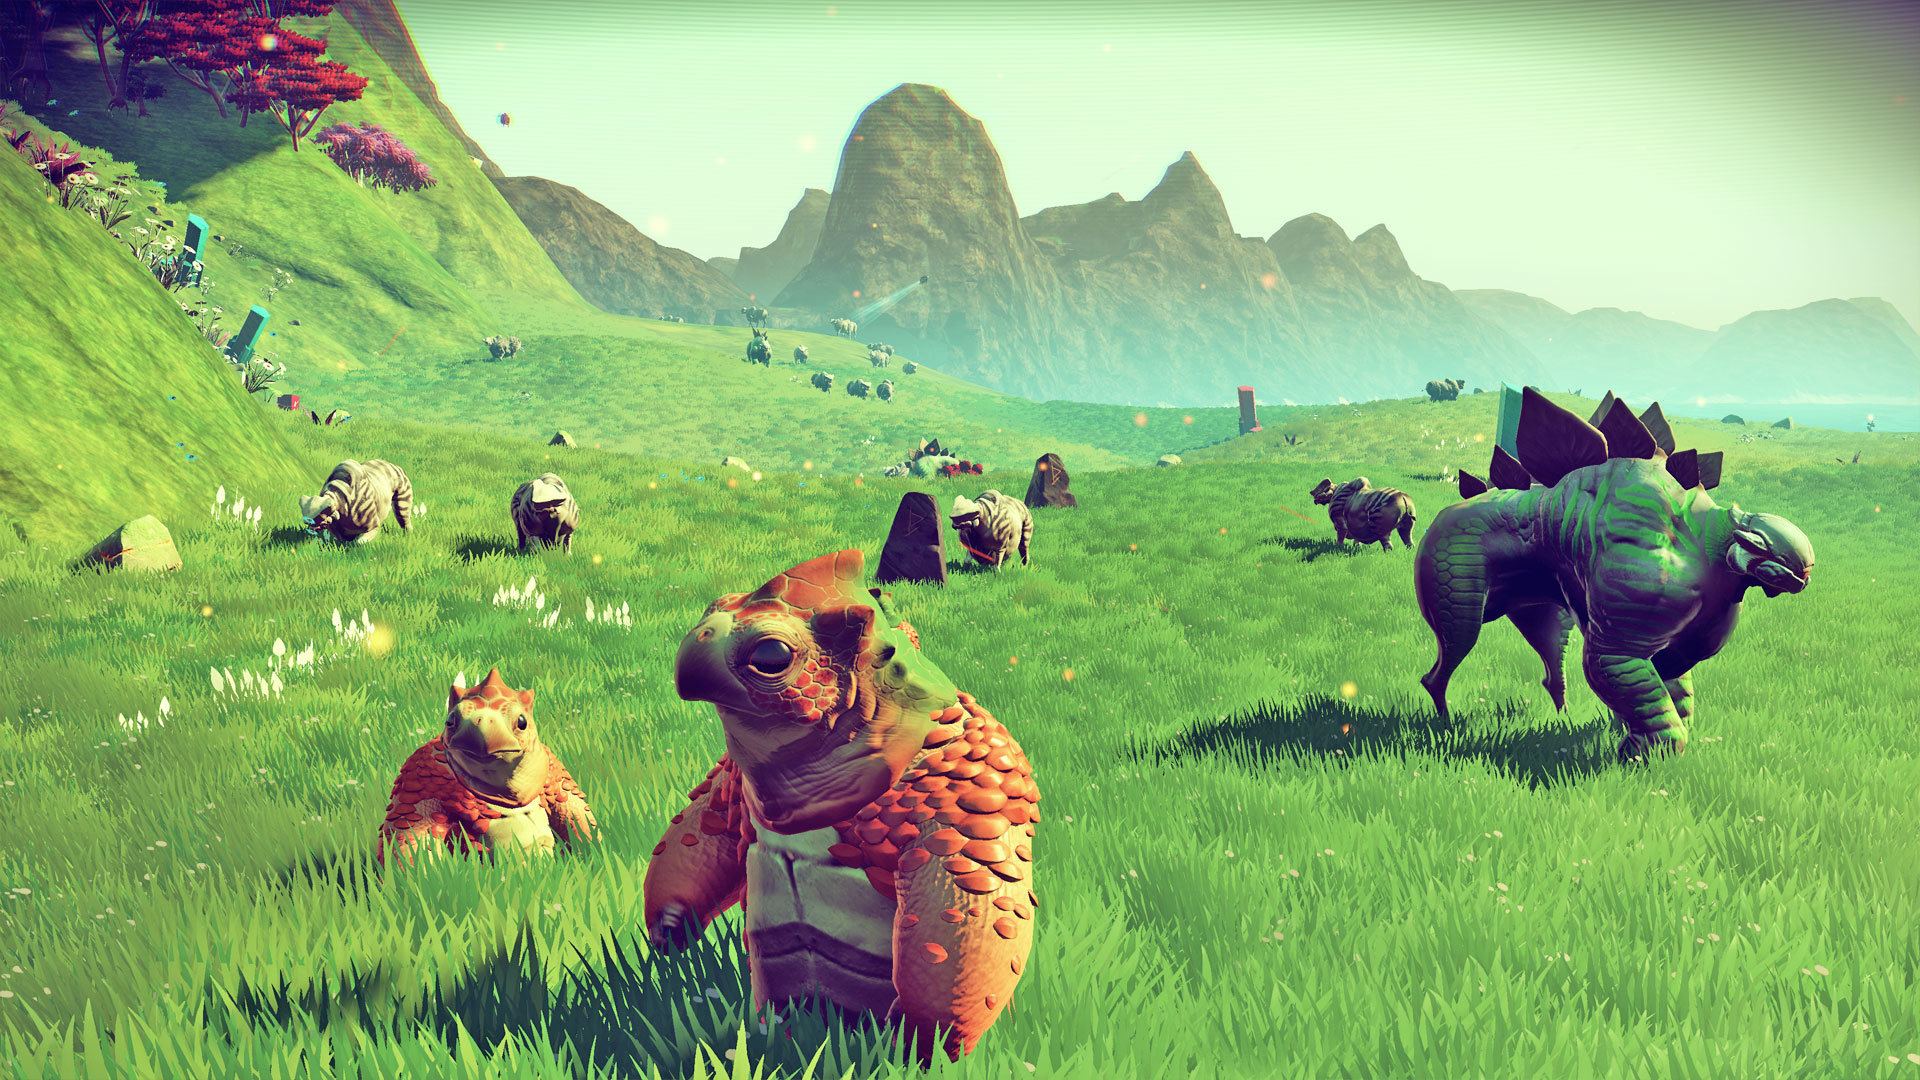
\includegraphics[width=.9\textwidth]{section01/assets/screenshot_NoManSky.jpeg}
\caption[A screenshot of "No Man's Sky"]{\label{Screenshot NoManSky}A screenshot of "No Man's Sky"}
\end{figure}

Well-known techniques such as fractals, L-systems, Perlin noise, and others have been used to procedurally generate plants, terrain, and cityscapes. At this point, we have to introduce a well-known game: "Minecraft", which can produce massive worlds that are chock-full of little details, like elaborate cliff faces and waterfalls. And it relies on procedural generation, which automatically creates environments and objects that are at once random, but guided by rules that maintain a consistent logic. Mountains are always rocky and sprinkled with snow, for example, while the low lands are typically full of grass and trees. Figure \ref{Screenshot Minecraft} is a screenshot of "Minecraft".

\begin{figure}[htb]
\centering
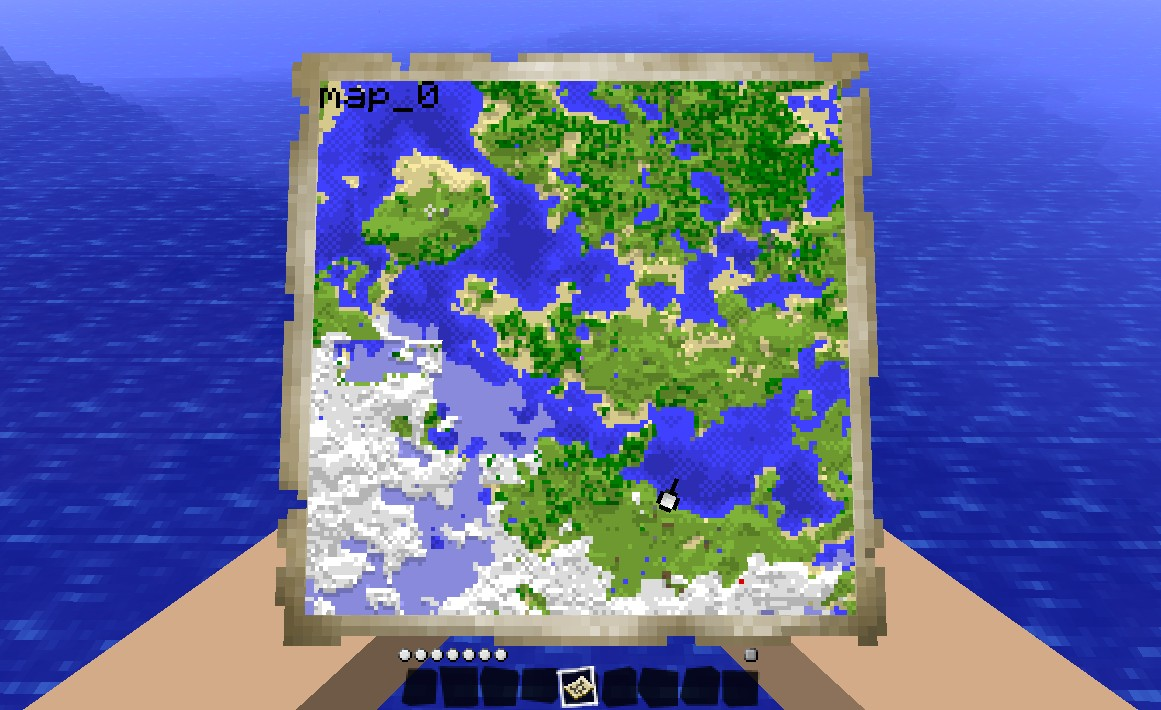
\includegraphics[width=.9\textwidth]{section01/assets/screenshot_Minecraft.jpg}
\caption[A screenshot of "Minecraft"]{\label{Screenshot Minecraft}A screenshot of "Minecraft"}
\end{figure}

\subsection{Similar Systems}
The "Medieval Fantasy City Generator(MFCG)" is a web application. This application generates a random medieval city layout of a requested size: small, medium or large, which is made up of different types of regions, and the generation method is rather arbitrary. Besides, many elements are provided for user to add to the city, such as farm fields, citadel, plaza, temple, river, coast and so on. Because of the premise of medieval fantasy, the map always includes the walls and castle, but the user can decide whether to display them. What's more, it allows the user to edit the map in order to modify some unsatisfying places using warp tool. The author also mentioned that the goal of the application is to produce a nice looking map, not an accurate model of a city. Finally, the user can save the map as an image in "png" or "svg" format by using the export feature if he is satisfied with the map. Figure \ref{Screenshot MFCG} is a screenshot of MFCG.

\begin{figure}[htb]
\centering
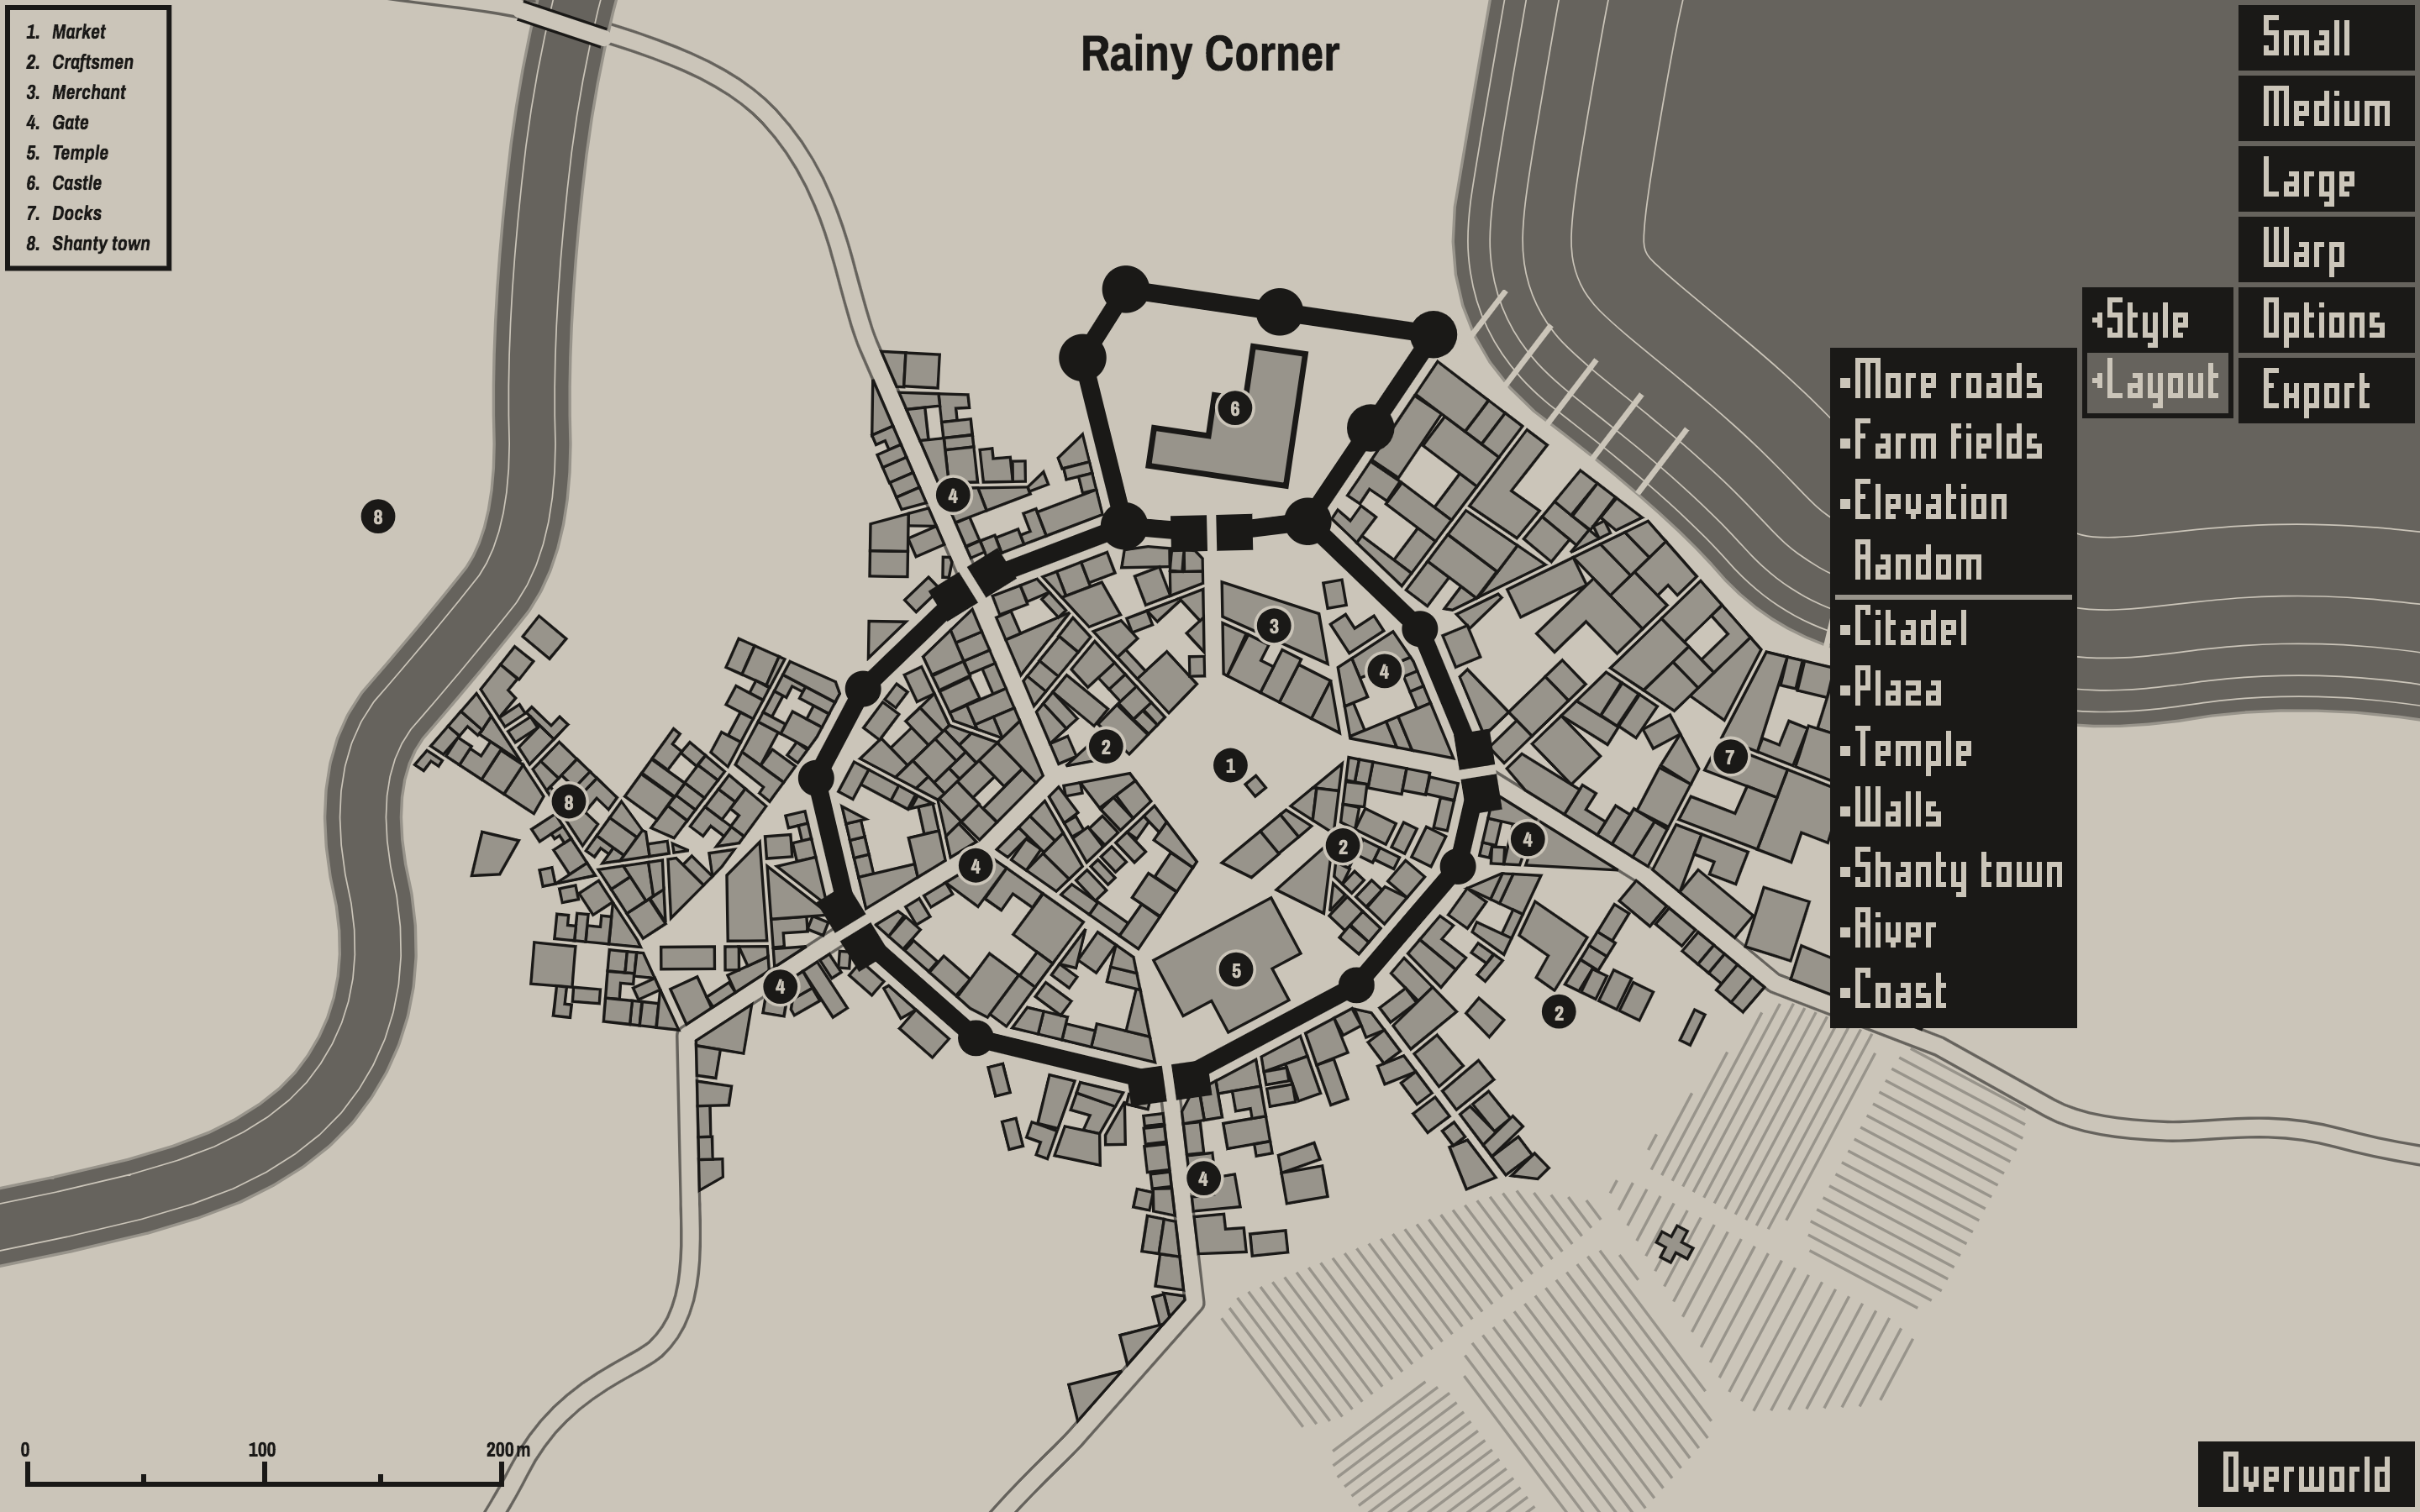
\includegraphics[width=.9\textwidth]{section01/assets/screenshot_MFCG.png}
\caption[A screenshot of Medieval Fantasy City Generator]{\label{Screenshot MFCG}A screenshot of Medieval Fantasy City Generator}
\end{figure}

The "Azgaar's Fantasy Map Generator(FMG)" is another similar system, which is a large scale system. The size of the map made by FMG varies from western Europe to the world continent, not just an island, but a random fantasy map represents pseudomedieval world.
Just like the real world, the map generated by FMG has the feature that the continent is always surrounded by the ocean and will never touch the border of the map. Although it is a random map, it is still based on real-world rules. While its biggest feature is that the user can choose the type of map he likes, which provides the following 5 types: political map, cultural map, height map, biomes map and pure landmass. In addition, it also supports user-defined map type, the user can add additional layers on existing map layer, such as: rivers layer, temperature layer, and population layer. What's more, it also allows the user to annotate and edit the map using layout editor, style editor, template editor, scale editor, countries editor, cultural editor or namebase editor. Last but not least, it supports exporting the map in "png" or "svg" format, but unlike the previous application, if the user wants to come back to edit the map in the future, he can save it in the "map" format. Figure \ref{Sample Map 1} is a screenshot of FMG.

\begin{figure}[htb]
\centering
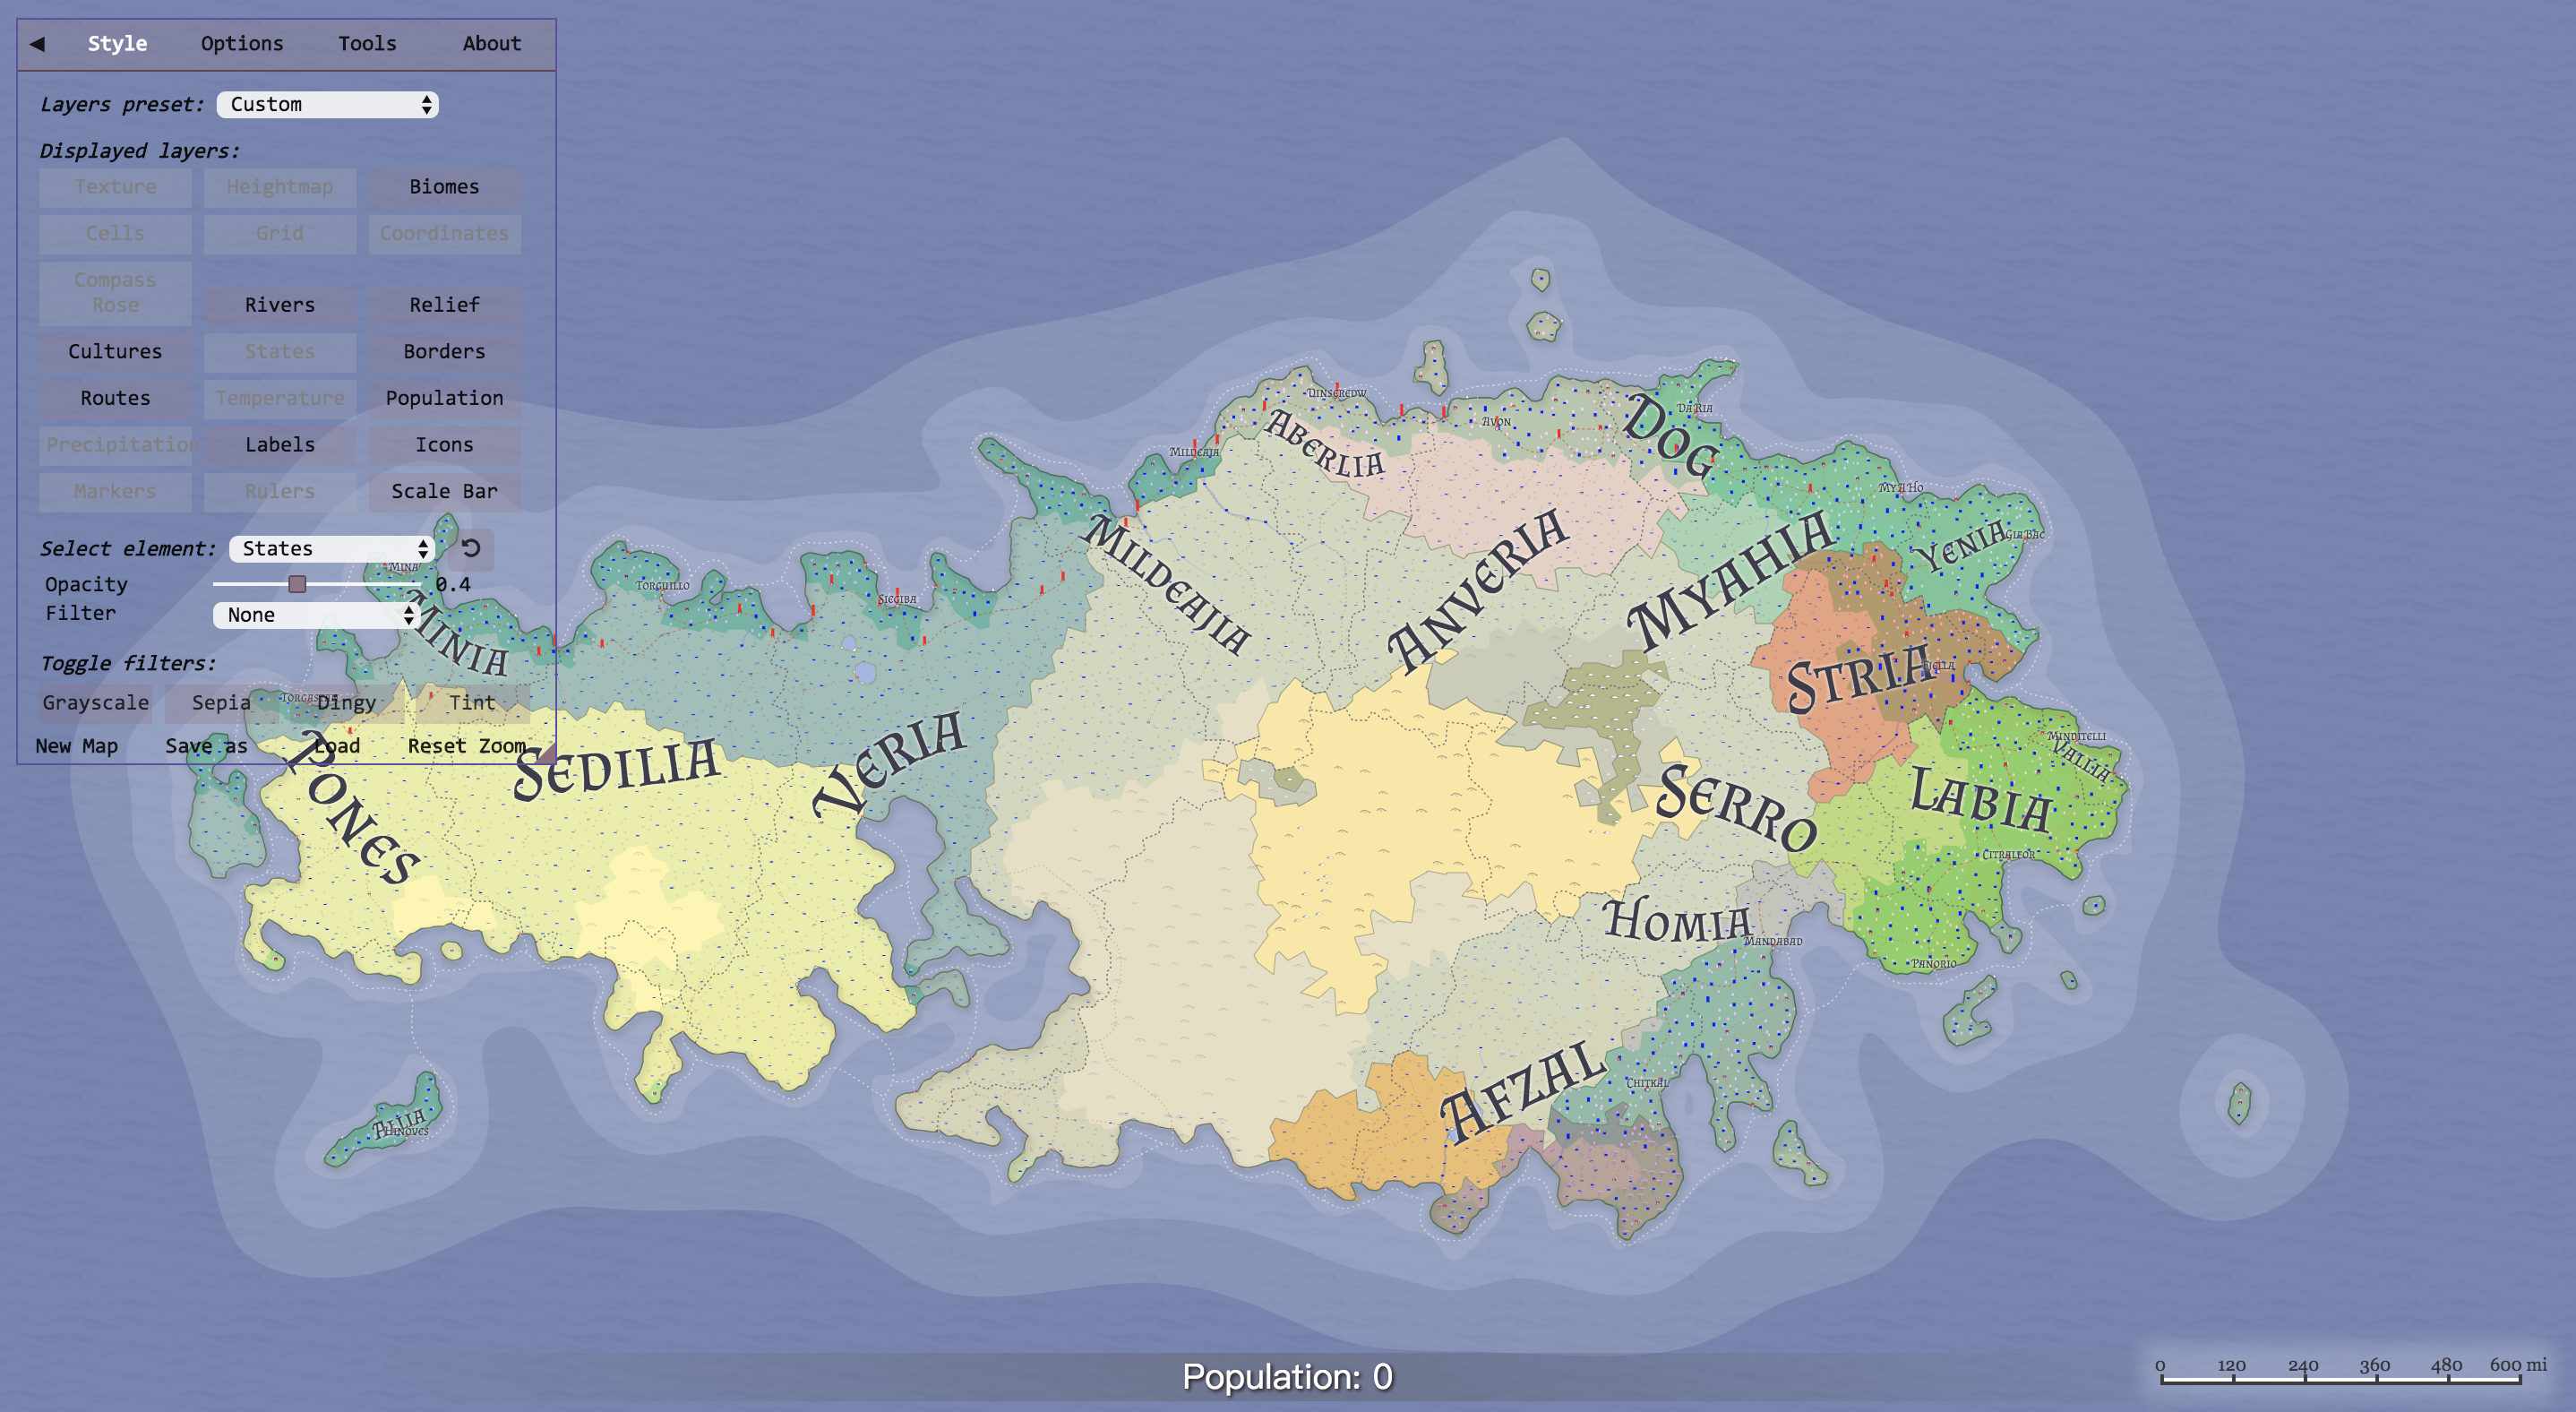
\includegraphics[width=.9\textwidth]{section01/assets/screenshot_FMG.png}
\caption[A screenshot of Azgaar's Fantasy Map Generator]{\label{Sample Map 1}A screenshot of Azgaar's Fantasy Map Generator}
\end{figure}

\subsection{Project Goal}
This project seeks to develop a software system that allows the user to generate maps of medieval cities for use in fantasy games or for purely artistic purposes. While the ultimate goal of this project is to procedurally replicate maps of a quality similar to the best cartographic hand-created maps by expert artists, we expect to obtain a modest approximation to the desired level of quality. Besides, our system will have the basic features such as: procedurally and randomly generated, allowing the user to annotate or edit, supporting the user to export map as an image in "png" or "svg" format, allowing the user to save it to the database and restore it from the server. In order to achieve these goals, we will implement the following operations and rules:
\begin{itemize}
	\item When the user open the map editor, it shows user an empty map with random map seeds by default, then the user can starting making map by accessing the menu on the right
	\item In the menu, the user can enter the number of map seeds to create a new empty map, or remain unchanged
	\item The user can choose the type of layout for the map: elevation, affluence, desirability, district and building, which can be superimposed on each other
  \item The user can choose to display street names or not
  \item The user can manipulate the "increase/decrease toggle", "increment sliding" and "waterline sliding" to edit the map: increasing or descreasing the value of elevation and affluence; building or removing the wall; making map cell as water or city
  \item If the waterline is changed, the continent will be changed accordingly
  \item The user can choose to display contour lines or not
  \item After selecting one or more than one layers under "edit" mode, the user can change the size of the "soft brush" by using the mouse wheel, which determines the area where the map will be edited
  \item The user edits the map by clicking and dragging the "soft brush"
  \item The districts and buildings are procedurally generated
  \item Besides, the user is allowed change the type of the current district by right clicking and selecting the context menu
  \item The map are divided into different types of districts: rich, medium, poor, empty, plaza, park, farm, water, harbor, university, religious, castle and military
  \item The user can zoom in and zoom out the map by pressing on the alt key and using the mouse wheel, of course, the map can be resized by a specialised button
  \item The user can save map or download it by clicking the button on the right bottom
\end{itemize}
